
\chapter{Gas-phase Metallicity and Radial Gradients in an Interacting System at $z \simeq 2$}

\section{Introduction}\label{sec:intro}

Galaxy gas-phase metallicities encode information about the history of gas accretion, star formation, and gaseous
outflows. Measurements of metallicity combined with accumulated stellar mass and gas content therefore provide
stringent constraints on the baryonic processes relevant to galaxy formation. Current observations show that
essentially all galaxies have low gas-phase metallicities compared to estimated chemical yields from star
formation, with greater discrepancy at lower stellar masses \citep[the mass-metallicity relation,
e.g.,][]{Tremonti2004, Lequeux1979}. This is commonly attributed to outflows of metal-enriched gas driven by
intense star formation, supported by observations that such feedback is ubiquitous among galaxies with high
densities of star formation \citep{Heckman2001, Newman2012}.  The \emph{spatial} distribution of metallicity
within a galaxy further constrains the baryonic assembly history, in particular the effects of outflows and
dynamical evolution. Star-forming disk galaxies in the local universe have negative radial metallicity gradients
(higher metallicity in the central regions; see \citealt{Sanchez2014} and \citealt{Vila-Costas1992} for large
samples). This has been explained by models of chemical evolution in which galaxies grow \emph{inside-out} such
that outer regions have younger characteristic ages \citep[e.g.,][]{Nelson2012}. Gradients typically flatten at
large radii indicating efficient mixing in those regions, possibly due to secular dynamical evolution or
recycling of metal-enriched gas which was previously ejected in outflows \citep[so-called "galactic fountains";
e.g.][]{Werk2011, Bresolin2012}. Notably, galaxies which are undergoing mergers or strong interactions have
significantly shallower metallicity gradients than isolated disks, which is understood numerically in terms of
radial gas flows induced by tidal forces \citep{Rupke2010a, Rupke2010b, Sanchez2014, Rich2012}.

This work is concerned with using time evolution of metallicity gradients as a probe of galaxy formation. We seek
to measure how gradients evolve, and to understand what processes drive that evolution. A variety of predictions
have been made based on numerical models of inside-out growth, ranging from steeper to flatter to inverted
(positive) gradients at higher redshifts \citep[e.g.,][]{Prantzos2000, Chiappini2001, Magrini2007, Fu2009}.
Cosmological simulations have recently begun to address this issue, with several groups arguing that gradient
evolution depends strongly on star formation feedback: stronger feedback is predicted to cause flatter gradients
due to rapid gas recycling \citep{Pilkington2012, Gibson2013, Angles-Alcazar2014}. Meanwhile the observational
results at high redshift have grown in number but comprise a variety of conclusions for the evolution of
gradients. Data reaching $\lesssim1$ kpc resolution with adaptive optics (and up to $\sim$100 pc in the case of
lensed galaxies) have revealed negative radial gradients with slopes often steeper than local descendants,
suggesting that gradients flatten as galaxies grow with time \citep{Jones2010,Jones2013,Yuan2011,Swinbank2012}.
Larger surveys with seeing-limited resolution of $\sim$5 kpc have reported mostly flat gradients with a
significant fraction of positive slopes \citep{Cresci2010,Queyrel2012,Stott2014,Troncoso2014}. These have been
interpreted as evidence for predicted "cold flows" of pristine gas
\citep[e.g.,][]{Dekel2009,Keres2009,Faucher-Giguere2011}, but these results are in contrast with high-resolution
measurements.

The discrepancy in metallicity gradient measurements at high redshift must be addressed in order to reliably
understand the role of gas and metal transport in galaxy evolution. High spatial resolution is clearly an
advantage; \citet{Yuan2013} demonstrate how degraded resolution can dramatically bias gradient measurements. For
typical-size galaxies at high redshift, $\lesssim1$ kpc resolution is essential to sample the scale radius and
reliably measure gradient slopes. The use of single strong-line metallicity indicators such as NII$/$\Ha\
\citep[e.g.,][]{Pettini2004} is another potential problem. Multiple emission line diagnostics are necessary  to
confirm variations in metallicity \citep[e.g.,][]{Jones2013} and to distinguish HII\ regions from AGN or shock
excitation, which in many cases are non-negligible \citep{Wright2010,Yuan2012,Newman2014} and would bias the
inferred gradients. In essence we require larger samples with high spatial resolution and a reliable suite of
metallicity and excitation diagnostics in order to resolve the discrepancy in existing measurements. Here we
present initial results from the \emph{Grism Lensed-Amplified Survey from Space} (GLASS) in which we measure
metallicities at $z\simeq2$ based on 5 nebular emission lines with resolution as fine as 200 pc. As with
\citet{Jones2013} this is enabled by a combination of strong gravitational lensing, broad wavelength coverage,
and diffraction-limited data. These results demonstrate the potential of the full GLASS survey to obtain dozens
of such measurements at $1.3\lesssim z \lesssim2.3$ and thus reliably determine the average evolution of
metallicity gradients over the past 11 Gyr.

Throughout this paper we adopt a flat $\Lambda$CDM cosmology with $\Omega_{\Lambda}=0.7$, $\Omega_{\rm M}=0.3$,
and $H_0=70$ \Hunit. At $z=1.85$, 3.5 Gyr has elapsed since the big bang and 1 arcsecond corresponds to 8.4 kpc
(c.f. 3.5 Gyr and 8.7 kpc/arcsecond for the \citealt{Planck2013} cosmology). All stellar masses (M$_*$) and star
formation rates (SFR) correspond to a \cite{Chabrier2003} initial mass function. Unless stated otherwise,
"metallicity" refers to the gas-phase oxygen abundance.


\section{A Triple Galaxy System at $z=1.855$}

The first GLASS observations of MACS J0717+3745 (hereafter \clyi) revealed three strongly lensed galaxies at the
same redshift $z=1.855\pm0.01$ (arc systems 3, 4, and 14 in \citealt{Schmidt2014}). The grism observations cover
three magnified images of each galaxy (e.g., arcs 3.1, 3.2, and 3.3 are multiple images of the same source) and
we list details of each image in Table~\ref{tab:magrslt}. The gravitational lensing model discussed in
Section~\ref{sec:model} indicates projected galaxy separations of 50 kpc for pairs 4--14, 150 kpc for 3--14, and
200 kpc for 3--4. Although the grism redshifts cannot constrain their line-of-sight separation to better than a
few Mpc, Keck/LRIS spectra of arcs 3.2 and 14.1 \citep{Limousin2012} and a Keck/MOSFIRE spectrum of arc 4.1
\citep{Schmidt2014} indicate consistent redshifts, corresponding to $\lesssim1$ Mpc in the Hubble flow. Therefore
all three galaxies appear to be physically associated. The fortuitous inclusion of these systems within \hst's
field of view, and the availability of several strong emission lines in the grism spectra, provide a laboratory
for studying how gas and heavy elements cycle within galaxies and their surrounding medium in an overdense
environment.


\section{Observations and Data Analysis}\label{sec:data}

Details of the GLASS survey design and grism spectroscopy are given in \citet{Schmidt2014}. Briefly, J0717 was
observed at two different position angles separated by approximately 100 degrees. The total exposure time is 10
orbits in the G102 grism and 4 orbits in the G141 grism. Data from each position angle are interlaced to produce
2D grism spectra and direct images with a scale of 0\farcs065 per pixel, Nyquist sampling the point spread
function. Direct images are used to estimate continuum spectra by dispersing each pixel from individual objects
detected in \sex \citep{Bertin1996} segmentation maps; these are used to guide the extraction of
individual object spectra and to subtract an estimate of the contamination from nearby objects.

The critical analysis method for this work is extraction of emission line maps. For each object of interest, we
use the direct image to construct a segmentation map and shift this to the expected wavelength of strong emission
lines using spectroscopic redshifts from the grism data (Figure~\ref{fig:spec2d}). We extract two-dimensional
maps of emission line flux and uncertainty for the region defined by the segmentation map, and correct for
residual background structure by subtracting a corresponding map at a nearby line-free wavelength (e.g., a
rest-frame 4750 \AA map is typically used to correct \Hb for imperfect continuum and contamination estimates).
Data affected by strong contamination are masked and treated as missing. We align the emission line maps
extracted from both position angles using bilinear interpolation, and combine them with an inverse-variance
weighting. Example emission line maps are shown for arc 4.1 in Figure~\ref{fig:spec2d_arc4}.

The \Hb and \OIII emission lines require special treatment in cases where  the spatial extent is sufficiently
large that these lines overlap. In all cases there is a region of pure \OIII $\lambda$5007 emission at the
rightmost edge of the blend (of $\simeq 6$ pixels or $0\farcs4$ in the dispersion direction for $z=1.855$). We
use the intrinsic flux ratio $f_{5007}/f_{4959} = 3$ to subtract the corresponding \OIII $\lambda$4959 flux,
which leaves another region of pure \OIII $\lambda$5007 emission. We iterate this process to completely de-blend
the \OIII doublet, resulting in separate $\lambda$4959 and $\lambda$5007 emission line maps. Additionally we
de-blend \OIII $\lambda$4959 and \Hb, although we cannot completely de-blend the lines in cases where \OIII
$\lambda$5007 and \Hb overlap. For $z=1.855$ this occurs whenever the source size is $\geq 1\farcs4$ in the
dispersion direction (for example, the spectrum of arc 14.1 shown in Figure~\ref{fig:spec2d}). In such cases we
treat the region where \OIII $\lambda$5007 and \Hb overlap as missing data.

\begin{figure}
    \centering
    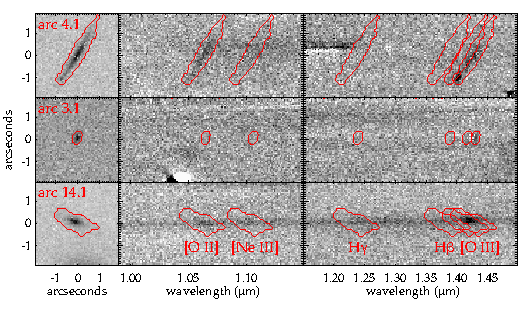
\includegraphics[width=\textwidth]{figures/figure_arcs_spectra_v2.pdf}
    \caption[Grism spectra for the arcs of interest show multiple spatially extended emission lines.]{Grism spectra for the arcs of interest show multiple spatially extended emission
    lines which can be used to derive metallicity maps. From left to right, each row shows the F140W direct
    image, G102 grism spectrum, and G141 grism spectrum. In all cases the estimated contamination has been
    subtracted from the spectra. Strong source continuum is apparent for arc 14.1. Red contours show the object
    segmentation maps derived using the direct images, and mapped to emission lines of interest in the grism
    spectra using the redshift of each source (left to right: \OII $\lambda\lambda$3727, \NeIII $\lambda$3869,
    \Hg, \Hb, \OIII $\lambda$4959, \OIII $\lambda$5007). The redshift is $z=1.855$ for all cases shown here.
    \label{fig:spec2d}}
\end{figure}

\begin{figure}
    \centering
    \includegraphics[width=\textwidth]{figures/figure_arc41_linemaps.pdf}
    \caption[\hst image and emission line maps.]{\hst image (top right; RGB: WFC3/F160W, WFC3/F110W, ACS/F814W) and emission line maps of arc 4.1.
    The typical flux uncertainty in each pixel is $2 \times 10^{-18}$ $\Funit$ (1$\sigma$).
    \label{fig:spec2d_arc4}}
\end{figure}


\section{Gravitational Lensing Model}\label{sec:model}

An accurate gravitational lensing model is essential for reconstructing the source plane morphology of lensed
galaxies, and for combining the information form the multiple images. As one of the Frontier Fields, the
gravitational lensing potential of \clyi\ has been modeled by several groups using a variety of techniques, and
the results are publicly available\footnote{http://www.stsci.edu/hst/campaigns/frontier-fields/}. We compared the
results of all models for which we could derive deflection angle maps at the redshift of interest (those of
Brada{\v c}, CATS, Sharon, and Zitrin) to assess which is best suited to the purposes of this work. We note that
those models are aimed at producing a global description of the cluster and therefore their accuracy in the
vicinity of the lensed images of interest is expected to vary significantly between them. The Sharon version 2
model \citep{Johnson2014} produced the best results for our images, yielding the most precise inversion. The
precision of the inversion was evaluated by comparing for each set of multiple images the promixity of the
inferred source position, and the agreement beetween source plane flux and morphology.  However, even the best
global model produced significant residual differences between the reconstructed sources, requiring an additional
step, as described in the next paragraph.

In order to take full advantage of the multiple images of each arc system, we have developed a novel technique to
align all images in the source plane. This allows us to reduce the lensing-related uncertainties and combine the
data from multiple images to increase signal to noise ratio of the emission line maps. The full details of our
methodology will be presented by Wang et al. (2014, in prep); here we give only a brief overview. Essentially, we
are considering the global cluster model as an approximate first solution and we are seeking corrections to the
potential to improve the reconstruction. We assume that the corrections are small and can thus be described by a
local correction to the lensing potential  up to the first two orders of derivatives.  The first order term
consists of a correction to the deflection angle for each image. The second order term yields corrections to the
shear and convergence. The procedure has thus five free parameters per image. The optimal parameters are found by
requiring the source plane reconstructions of each set of multiple image to be as similar to each other as
possible. We note that a direct byproduct of this formalism is a correction to the magnification of each image.

We have applied this method to the arc systems 3, 4, and 14, using the least distorted (i.e., least magnified)
image of each system as a reference. Table~\ref{tab:magrslt} lists the local convergence and shear before and
after correction, and corrected magnifications. {\bf is this still true?} In all cases the corrected
magnification ratios are in better agreement with measured flux ratios with respect to the original methods. The
morphologies of the reconstructed sources are also in excellent agreement showing that the second order
correction is sufficient for our purposes.

In the following analysis we combine emission line maps from multiple images in the source plane in order to
increase signal to noise ratio. However, including less highly magnified images provides a marginal improvement
at the cost of degraded spatial resolution. We therefore use arcs 3.1$+$3.2, arc 4.1 only, and arcs 14.1$+$14.3
to optimize resolution and sensitivity. Final results are consistent with measurements from individual images.
Combining multiple images improves the precision in metallicity gradients by an impressive factor of
$\simeq2\times$ for arcs 3 and 14 by enabling finer spatial sampling and detection of more extended low surface
brightness emission.

We derive a conservative uncertainty of 13\% RMS in the magnification factors (prior to second order correction)
by comparing measured flux ratios of multiple images with model-predicted magnification ratios. This error is not
propagated in the following analysis, however it is small compared to other sources of uncertainty and has no
effect on the results.

\begin{figure}
    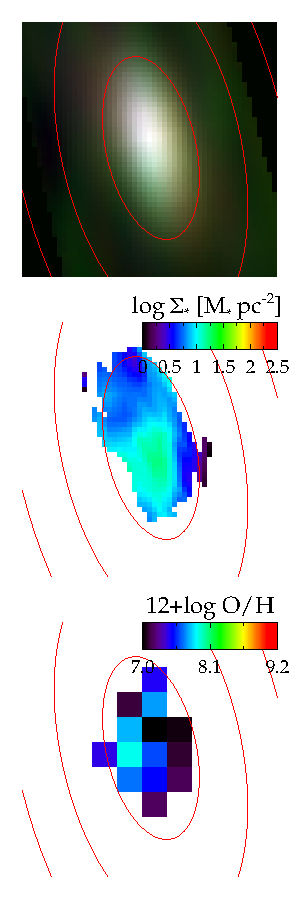
\includegraphics[width=.3\columnwidth]{figures/figure_arc3_source_corr.pdf}
    \hspace{0.03\columnwidth}
    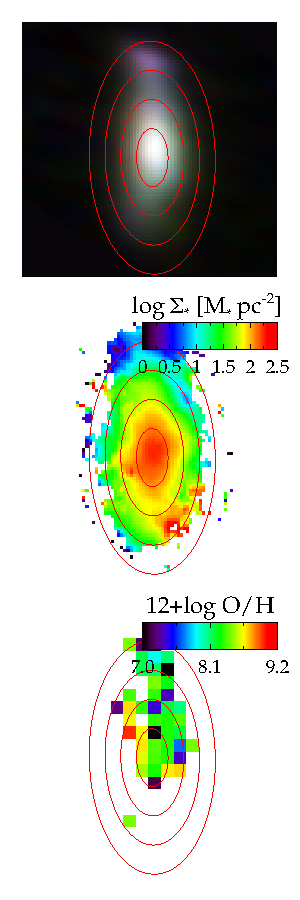
\includegraphics[width=.3\columnwidth]{figures/figure_arc4_source_corr.pdf}
    \hspace{0.03\columnwidth}
    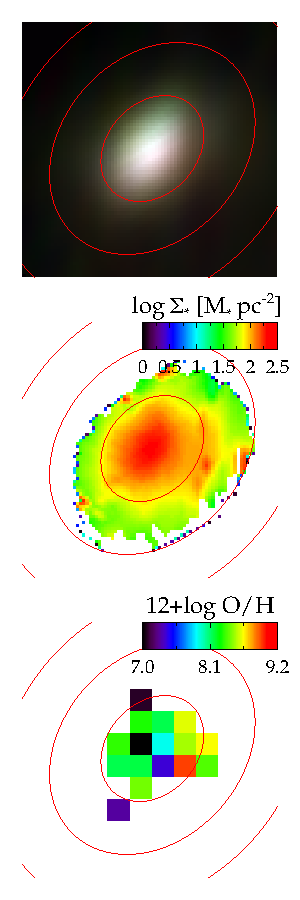
\includegraphics[width=.3\columnwidth]{figures/figure_arc14_source_corr.pdf}
    \caption[Source plane morphologies of arcs 3, 4, and 14.]{
    \label{fig:sourceplane}
    Source plane morphologies of arcs 3, 4, and 14 (from left to right). Each panel shows contours of constant de-projected galactocentric radii at intervals of 1 kpc, derived in Section~\ref{sec:properties}.
    \emph{ Top row:} \hst\ image (RGB: WFC3/F160W, WFC3/F110W, ACS/F814W).
    \emph{ Middle:} stellar mass maps derived from spatially resolved \hst\ photometry. All galaxies have smooth, centrally peaked stellar mass profiles with no significant secondary peaks.
    \emph{ Bottom:} gas-phase metallicity maps.
    }
\end{figure}


\section{Physical Properties}\label{sec:properties}

\subsection{Stellar Mass}\label{sec:mstar}

We use version 1.0 of the stellar population synthesis code FAST \citep{Kriek2009} to fit the resolved spectral
energy density (SED) of each galaxy of interest. For $z=1.855$, the rest-frame UV through optical SEDs are well
constrained by broad-band \hst\ photometry taken as part of the CLASH survey \citep{Postman2012}. We utilize the
ACS/F435W, ACS/F606W, ACS/F814W, and WFC3/F125W filters which sample nearly the full rest-frame wavelength range
from 1250--4900 \AA. This set of filters is chosen to provide the widest possible wavelength coverage while
avoiding contamination from the strong emission lines \lya, \OII, and \OIII which can significantly affect the
broad-band photometry and derived stellar population properties. In particular, \OIII emission accounts for
$\sim$25\% of the total WFC3/F160W flux (an increase of 0.3 magnitudes) for the galaxies discussed here.

Our methodology is as follows. We first align all images with the GLASS F105W direct image and smooth to a common
point spread function of 0\farcs2 FWHM. The broad-band fluxes in each pixel are fit with a \citet{Bruzual2003}
stellar population library, \cite{Chabrier2003} initial mass function, Milky Way dust attenuation law, stellar
ages between 5 Myr and the age of the universe at the galaxy's redshift, and an exponentially declining star
formation history with $\tau = 10^{7}-10^{10}$ yr. The quantity of greatest interest is the derived stellar mass
surface density, which is the most robust parameter. Other stellar population parameters (SFR, age, extinction,
etc.) are obtained simultaneously albeit with larger uncertainty. We have repeated the SED analysis using
additional broad-band filters corrected for emission line contamination using the flux maps described in
Section~\ref{sec:data}, verifying that this produces consistent results. Total stellar masses derived from
integrated photometry and corrected for magnification are listed in Table~\ref{tab:arcs}.


\subsection{Morphology}\label{sec:morphology}

Morphological information is critical for measuring accurate metallicity gradients, as the radial coordinate
depends on a galaxy's central position and inclination. Ideally the dynamical center, major axis orientation, and
inclination would be constrained from kinematics as has been done for previous work \citep[e.g.,][]{Jones2013},
but we lack kinematic data. Instead we derive estimates of these quantities by assuming that the stellar mass
surface density derived in Section~\ref{sec:mstar}, $\Sigma_*$, is elliptically symmetric. We reconstruct
$\Sigma_*$ using the lens model (Section~\ref{sec:model}) and fit for the centroid, orientation, and axis ratio.
Only the most highly magnified image in each arc system is used in order to maximize the spatial resolution. In
the following analysis we adopt the galaxy center and inclination such that contours of $\Sigma_*$ trace contours
of constant de-projected radius.

Source plane $\Sigma_*$ distributions and best-fit ellipses are shown in Figure~\ref{fig:sourceplane}. All
galaxies exhibit smooth, centrally peaked stellar mass profiles with contours that are fit by ellipsoids. Within
the stellar mass uncertainty, we find no evidence for ongoing late-stage major mergers which could manifest as a
secondary peak in the stellar mass density.


\subsection{Metallicity and Nebular Extinction}\label{sec:z}

We use the strong line ratio calibrations presented by \cite{Maiolino2008} to estimate gas-phase oxygen abundance
(expressed as \oh) and nebular extinction A(V) from measured \OII, \NeIII, \Hg, \Hb, and \OIII fluxes. We use a
\cite{Cardelli1989} extinction curve with R$_{\rm V} = 3.1$, noting that the choice of R$_{\rm V}$ has no
significant effect on the derived metallicity (typically $<0.1$ dex for $2\leq {\rm R_V} \leq 5$).  To further
constrain A(V), we impose $\frac{\rm{H}\gamma}{\rm{H}\beta} = 0.47$ as expected for Case B recombination and
typical \HII\ region conditions \citep[e.g.,][]{Hummer1987}.  Metallicity and extinction are derived from a
$\chi^2$ statistic constructed from all available diagnostics: $$\chi^2 = \sum_R \left[ \frac{\Delta
R}{\sigma(R)} \right]^2.$$
%
Here $\Delta R$ is the difference between predicted and observed de-reddened flux ratios at a given A(V) and \oh,
and the uncertainty $\sigma(R)$ includes RMS scatter in each calibration added in quadrature with measurement
uncertainty. We adopt the best fit as the values that minimize $\chi^2$, and 1$\sigma$ uncertainty from the
extrema at which $\chi^2$ differs by 1 from the minimum value. This is slightly smaller than the formal
uncertainty because of covariance between various metallicity diagnostics are independent; we have checked that a
more careful treatment does not affect the results. We limit the solutions to A(V)~$=0-3$ and \oh~$=7.0-9.3$
\citep[equivalent to $0.02-4.1\times$ the solar abundance of \oh~$=8.69$;][]{Allende2001}. While the formal
best-fit solutions are occasionally beyond this range, all such cases are poorly constrained and we view such
extreme conditions as highly unlikely. Although the extinction is poorly constrained for most individual pixels,
SED fitting (Section~\ref{sec:mstar}) and averaged \Hb$/$\Hg\ ratios indicate relatively low extinction toward
both the stars and \HII\ regions, with best-fit A(V)$=0-0.6$ and permitted A(V)$<1.1$ (1$\sigma$) in the dustiest
case. Fortunately, uncertainty in extinction has little effect on the derived metallicity since many diagnostic
line ratios are relatively insensitive to reddening.

Maps of the source plane gas-phase metallicity are shown in Figure~\ref{fig:sourceplane}. The emission line maps
are binned to spatial scales of $\simeq300-500$ pc and the metallicity is fit for all such pixels where at least
one emission line is detected at $\geq 5\sigma$ significance. All sources are well resolved with measurements
extending over $\simeq3$ resolution elements for arc 3, and $\geq 6$ resolution elements for the others. The
metallicity is typically sub-solar with most pixels having best-fit \oh\ in the range 7.5$-$8.5, corresponding to
flux ratios $\frac{\rm [O~\textsc{iii}]}{\rm{H} \beta} > 2.5$ and $\frac{\rm [O~\textsc{iii}]}{\rm
[O~\textsc{ii}]} > 1$. Figure~\ref{fig:sourceplane} also shows several pixels for which the best-fit metallicity
is at the extreme ends of the permitted range; these usually correspond to noise artifacts and/or single-line
detections and are therefore unreliable.

In addition to the spatially resolved analysis, we calculate galaxy-averaged metallicity and extinction by
applying the same analysis to total emission line fluxes measured from integrated 1-D spectra. The results agree
with the average of individual pixel values (Table~\ref{tab:arcs}), providing a valuable sanity check. The
slightly lower average metallicity of individual pixels c.f. integrated flux is likely due to the requirement of
a 5$\sigma$ detection of \OIII (the brightest emission line), which induces a bias toward lower metallicity.
Extinction-corrected Balmer line fluxes derived from this analysis are used to determine star formation rates in
Section~\ref{sec:sfr}.


\subsection{Metallicity Gradient}\label{sec:gradients}

Gas-phase metallicity gradients are derived from the morphology and metallicity analyses described in
Sections~\ref{sec:morphology} and \ref{sec:z}, respectively. We consider two measurements based on (1) individual
pixels and (2) radial binning. For the first method, we compute the gradient $\frac{\Delta Z}{\Delta R}$ from a
linear fit to the metallicity vs. de-projected radius of individual pixels (those shown in
Figure~\ref{fig:sourceplane}):
\begin{equation}\label{eq:gradient} 
    \oh = Z_0 + \frac{\Delta Z}{\Delta R} R.
\end{equation}
This functional form is a good fit to the data and we are unable to distinguish more complex
behavior given the measurement uncertainties. Pixels for which the allowed (1$\sigma$) range of \oh\ extends to
$\leq7$ or $\geq9.3$ are excluded from the fit as these are generally unreliable and have large uncertainty
($\gtrsim 1$ dex), although including these data gives consistent results. For the second method we bin the
emission line flux in annular apertures for each source, calculate metallicity from the total flux in each
aperture, and compute the gradient using Equation~\ref{eq:gradient}. The range of radii for each annulus is
chosen to provide a $\simeq10\sigma$ detection of \OIII, which is uniformly the strongest emission line. We show
the data and best-fit gradients in Figure~\ref{fig:gradients} and list the results in Table~\ref{tab:arcs}.
Uncertainty in inclination and magnification are not included in these error estimates, but these effects are
small ($\lesssim 30$\% combined) compared to uncertainty in the metallicities.

Both methods of calculating the metallicity gradient use the same diagnostics applied to the same data set and
give consistent results. The pixelated approach is similar to local galaxy measurements which are based on
individual \HII\ regions \citep[e.g.,][]{Vila-Costas1992}, and the radial binning method is equivalent to most
measurements reported for high redshift galaxies \citep{Yuan2011,Swinbank2012,Queyrel2012,Stott2014}. The primary
differences are that the annular binning method is higher signal to noise ratio and is spatially complete,
whereas low surface brightness regions are either noisy or excluded from the pixelated method. We therefore
consider the annular binning method to be more robust.


\begin{figure}
    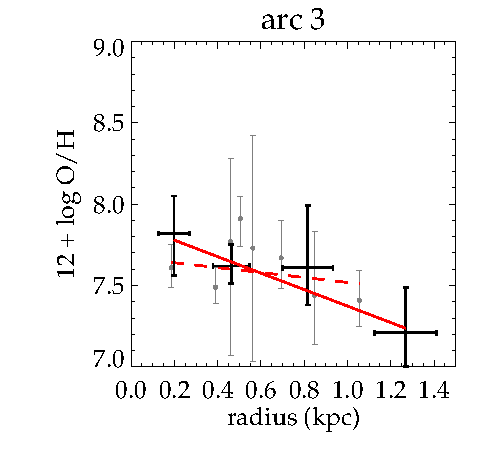
\includegraphics[width=.33\textwidth]{figures/figure_arc3_gradient_bin_corr.pdf}
    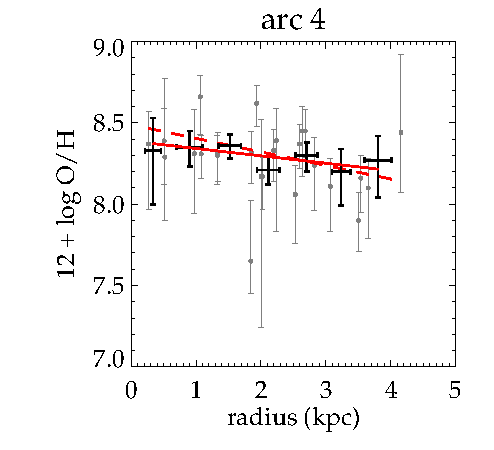
\includegraphics[width=.33\textwidth]{figures/figure_arc4_gradient_bin_corr.pdf}
    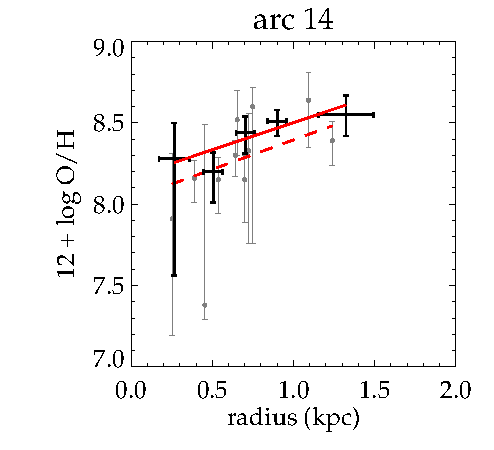
\includegraphics[width=.33\textwidth]{figures/figure_arc14_gradient_bin_corr.pdf}
    \caption[Radial metallicity gradients in each galaxy.]{ \label{fig:gradients} Radial metallicity gradients in each galaxy. Grey points are measured from
    individual source plane pixels shown in Figure~\ref{fig:sourceplane}, and thick black points show the results
    for flux summed within radial annuli. Linear gradient fits to the individual pixels and radial bins are shown
    as dashed and solid lines, respectively. Both methods give consistent results.}
\end{figure}



\subsection{Star Formation Rate}\label{sec:sfr}

Star formation rates are derived from Balmer emission using standard methods. We convert the extinction-corrected
total \Hb flux (Section~\ref{sec:z}) to SFR following \cite{Kennicutt1998}, divide by 1.7 to convert to a
\cite{Chabrier2003} IMF, and divide by the lensing magnification to recover the intrinsic SFR of each galaxy.
Results are given in Table~\ref{tab:arcs} including uncertainty from measurement noise and extinction. Additional
uncertainties associated with the choice of $R_V$ and underlying stellar absorption (for which we make no
correction) are negligible.


\subsection{AGN Contamination}

In calculating metallicities and SFR we have assumed that all nebular emission arises in \HII\ regions. The
presence of shocks or AGN can bias these results even for very weak nuclear sources and we therefore check for
any possible contamination. The global flux ratios of each galaxy, as well as the individual annular bins shown
in Figure~\ref{fig:gradients}, are consistent with \HII\ regions. However in all cases the line ratios fall in
the region occupied by both \HII\ and AGN excitation \citep[such as the "blue" diagnostic diagram,
e.g.,][]{Lamareille2010}, and we lack a low-excitation line such as \NII or \SII which would permit more
reliable classification \citep[e.g.,][]{Jones2013}. Publicly available Chandra/ACIS data\footnote{Available at
http://cxc.cfa.harvard.edu/cda/} show no X-ray detection for any of the arcs, and all three arcs have
moderate-resolution Keck spectra which show no sign of AGN features \citep{Schmidt2014,Limousin2012}. We note
that the central resolution element of arc 14 shows marginal evidence ($\sim2\sigma$) of an elevated \OIII$/$\Hb
ratio as expected for AGN \citep[e.g.,][]{Wright2010,Newman2014}.  \cite{Trump2011} have associated this signal
with a significant AGN fraction in stacks of galaxies of similar stellar mass and redshift whose individual X-ray
luminosities are below the detection threshold, although it is not a reliable indicator of AGN in individual
galaxies.  To summarize, we find no conclusive evidence of AGN but cannot rule out a possible low-level
contribution to the emission line flux from a nuclear source. The expected effect of such activity would be to
lower the derived central metallicity, with no significant effect on SFR or stellar masses.

%= = = = = = = = = = = = = = = = = = = = = = = = = = = = = = = = = = = = = = = =

\begin{deluxetable}{lcccccccc}
\tablecolumns{8}
\tablewidth{0pt}
\tablecaption{Source properties\label{tab:arcs}}

\tablehead{
\colhead{ID} & \colhead{$z$} & \colhead{log M$_*$}      & \colhead{SFR}          & \colhead{\oh\tablenotemark{1}} & \colhead{\oh\tablenotemark{2}} & \colhead{$\Delta \rm{Z} / \Delta \rm{R}$\tablenotemark{3}} & \colhead{$\Delta \rm{Z} / \Delta \rm{R}$\tablenotemark{4}} \\
\colhead{}   & \colhead{}    & \colhead{[log $\Msun$]}  & \colhead{[$\Msunyr$]}  & \colhead{}                 & \colhead{}                       & \colhead{[dex kpc$^{-1}$]}      & \colhead{[dex kpc$^{-1}$]} \\
}
\medskip
\startdata
arc 3   &  1.855  &  7.2$\pm$0.4          &  1.6$^{+1.0}_{-0.6}$  &  7.50$\pm$0.28  &  7.76$^{+0.25}_{-0.20}$  &  -0.15$\pm$0.23  &  -0.51$^{+0.36}_{-0.27}$  \\
arc 4   &  1.855  &  9.3$^{+0.2}_{-0.1}$  &  14.8$^{+21.3}_{-4.3}$  &  8.22$\pm$0.32  &  8.32$^{+0.12}_{-0.15}$  &  -0.08$\pm$0.04  &  -0.05$\pm$0.05  \\
arc 14  &  1.855  &  8.8$^{+0.2}_{-0.1}$  &  3.3$^{+3.2}_{-0.9}$  &  8.21$\pm$0.44  &  8.30$^{+0.15}_{-0.23}$  &   0.36$\pm$0.46  &   0.33$\pm$0.21  \\
\enddata
\tablenotetext{1}{Average and RMS scatter of individual pixels}
\tablenotetext{2}{Best fit and 1$\sigma$ uncertainty derived from integrated spectrum}
\tablenotetext{3}{Derived from individual pixels}
\tablenotetext{4}{Derived from total flux in radial apertures}
\end{deluxetable}


%= = = = = = = = = = = = = = = = = = = = = = = = = = = = = = = = = = = = = = = =


\section{Results and Discussion}\label{sec:results}

\subsection{Global Properties}

In this section we examine the GLASS sample studied here in the context of the general $z\simeq1.8$ galaxy
population, as a prelude to discussing the implications of our results for galaxy evolution.
Figure~\ref{fig:properties} summarizes the demographic properties compared to larger published samples at similar
redshift. Comparison samples are carefully chosen to minimize systematic effects: the narrow range of redshift
mitigates any evolutionary trends, all data points are calculated with the same IMF and stellar population
templates, and all stellar masses account for the contribution of emission lines to broad-band photometry.
Ignoring this last effect would result in higher stellar masses by $\simeq0.15$ dex for arcs 4 and 14 and
$\simeq0.6$ dex for arc 3, in excellent agreement with the mass-dependent estimates by \cite{Whitaker2014}. In
lieu of metallicity, we use \OIII$/$\OII flux ratios for a clear comparison of observable properties. While this
ratio is sensitive to metallicity, ionization parameter, and reddening, all of these quantities are intrinsically
correlated and vary monotonically with \OIII$/$\OII \citep[e.g.,][]{Maiolino2008,Dopita2013}. We can therefore
directly compare {\em relative} oxygen abundances between different samples, noting that secondary parameter
dependences result in $\simeq0.25$ dex RMS scatter between metallicity and \OIII$/$\OII.

In comparison to the overall population, the galaxies studied here have SFRs which are a factor of $\geq3\times$
above the "main sequence" locus of SFR and M$_*$ (Figure~\ref{fig:properties}). Such high relative SFRs are often
induced by gravitational interactions, and indeed \cite{Stott2013} show that $\sim50$\% of sources at this SFR,
M$_*$, and $z$ are merger events. The metallicities inferred from \OIII$/$\OII are consistent with comparison
samples of similar SFR and M$_*$, as are the nebular extinction values. The GLASS data are also consistent with a
steep mass-metallicity relation as found by \cite{Henry2013}, although the scatter in Figure~\ref{fig:properties}
is large. To summarize, the global properties are typical of low-mass starbursts at $z\simeq2$ which are
frequently associated with galaxy interactions.


\begin{figure}
    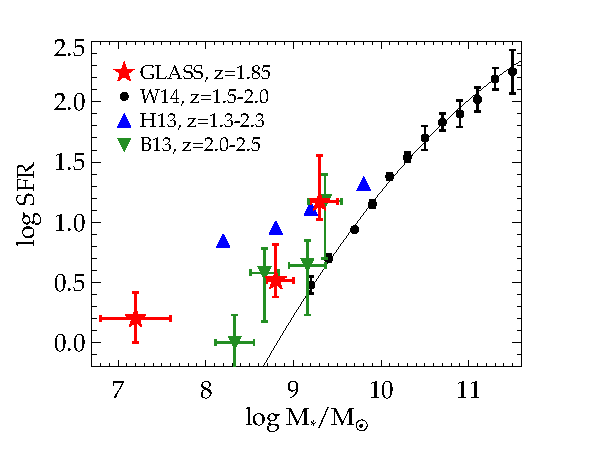
\includegraphics[width=.5\textwidth]{figures/figure_ms_corr.pdf}
    \includegraphics[width=.5\textwidth]{figures/figure_o32_corr.pdf}
    \caption[Global demographic properties of the GLASS arcs.]{Global demographic properties of the GLASS arcs. For comparison we also show average values of
    larger samples at similar redshift from WISP \citep[][H13]{Henry2013} and 3D-HST \citep[][W14]{Whitaker2014}
    data as well as individual lensed galaxies reported by \citet[][B13]{Belli2013}. \emph{ Top:} SFR versus
    stellar mass.  The arcs studied here have significantly higher specific SFR compared to the "main sequence"
    at $z\simeq1.8$ (shown by the W14 data), consistent with expectations for excess star formation triggered by
    gravitational interactions among these systems. \emph{ Bottom:} comparison of emission line ratios versus
    stellar mass. Open symbols show the effect of dust attenuation measured by \cite{Henry2013}; all other data
    are uncorrected for reddening. The arcs studied here have typical \OIII/\OII ratios for their redshift,
    stellar mass, and SFR. The right axis shows equivalent metallicity corresponding to \OIII/\OII for the
    \cite{Maiolino2008} calibration used in this work. The GLASS data are consistent with a steep
    mass-metallicity relation as found by \cite{Henry2013}, and notably extend to an order of magnitude lower in
    stellar mass compared to previous studies at $z\simeq2$.\label{fig:properties}}
\end{figure}


\subsection{Metallicity Gradient Evolution}

We now turn to a discussion of the metallicity gradient of arc 4 and its evolution with redshift.
Figure~\ref{fig:evolution} compares the GLASS data with similar measurements as a function of redshift. Arcs 3
and 14 are not included because their gradients are poorly constrained, due to their small physical sizes and
lower signal to noise ratio.  We restrict the comparison sample to measurements with $\lesssim1$ kpc resolution,
noting that even kpc resolution results in artificially flat inferred gradients for typical high redshift
galaxies \citep[e.g.,][]{Yuan2013,Stott2014}. We show original published values for all comparison data with the
caveat that they are derived using different strong-line calibrations; this has minimal effect on our conclusions
since metallicity gradients are relatively insensitive to the choice of calibration \citep{Jones2013}. However
none of the comparison data include scatter in metallicity in the formal uncertainty, hence the error bar on arc
4 is the most conservative of those shown in Figure~\ref{fig:evolution}.  Ideally we would construct a sample
which corresponds to approximately the same galaxy population \citep[as was done in][]{Jones2013}, but we are
presently limited by the available data at high redshift. The result is that arc 4 is expected to have $\sim0.4$
dex lower stellar masses at a given redshift than average sources in Figure~\ref{fig:evolution}, which are
approximately Milky Way analogs \citep[based on abundance matching; e.g.,][]{Behroozi2013}. Nonetheless this
provides a useful comparison.

Figure~\ref{fig:evolution} demonstrates that interacting galaxies (shown as open symbols) have flatter gradients
than isolated counterparts. This is most evident in the lensed and $z=0$ samples which have the best spatial
resolution. Here we include arc 4 as an interacting system. This is motivated by results which show dramatically
flattened gradients even in widely separated pairs (such as arcs 4--14) compared to an isolated control sample
\citep[][and references therein]{Rich2012}, as well as the enhanced SFR which suggest interaction-driven gas
flows. The relatively shallow metallicity gradient of arc 4 is therefore fully consistent with expected
gravitational interaction.

An alternative cause for the shallow gradient of arc 4 is metal mixing by strong feedback. To illustrate this,
Figure~\ref{fig:evolution} shows evolutionary tracks for two simulations with different sub-grid feedback
prescriptions of an otherwise identical Milky Way-like galaxy discussed by \cite{Gibson2013}, and we now briefly
summarize their findings. The "normal" feedback simulation \citep[MUGS;][]{Stinson2010} results in relatively
steep metallicity gradients of 0.2--0.3 dex\,kpc$^{-1}$ at $z\simeq2$ which flatten at later times. The MaGICC
simulation \citep{Brook2011} employs an enhanced feedback scheme, in which galactic outflows are more effective
at removing metal-enriched ISM material which is re-accreted preferentially in outer regions. This mixing of the
ISM results in shallower gradients of $<0.05$ dex\,kpc$^{-1}$ which become marginally steeper with time. The
enhanced feedback results are in excellent agreement with the shallow gradient measured for arc 4. Other groups
have found essentially identical results with various feedback mechanisms which act to redistribute energy and
ISM material throughout galactic disks \citep[e.g.,][]{Yang2012,Angles-Alcazar2014}. For the case of rapidly
recycled outflows we would expect a signature of higher overall metallicity, whereas gravitational interactions
should have an opposite effect \citep[e.g.,][]{Rich2012}. We note that \cite{Kulas2013} report evidence for rapid
recycling in a protocluster at $z=2.3$ based on stacked spectra, and we might expect a similar observational
signature in the overdense region studied here. However, the expected differences are small \citep[$\sim0.1$
dex;][]{Torrey2012,Kulas2013} compared to measurement uncertainties so we are unable to distinguish these
scenarios without additional complementary data. In any case the shallow gradient in arc 4 suggests that metals
are efficiently mixed throughout the ISM on scales of several kpc.


\begin{figure}
    \centering
    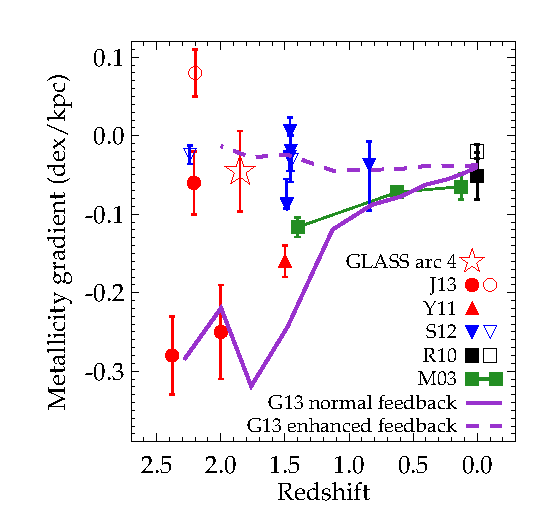
\includegraphics[width=.8\textwidth]{figures/figure_gradient_evolution_corr.pdf}
    \caption[Evolution of metallicity gradients with redshift.]{Evolution of metallicity gradients with redshift. We compare the gradient of arc 4 from this work
    with published measurements at high redshift including other lensed galaxies (\citealt{Jones2013}, J13;
    \citealt{Yuan2011}, Y11), non-lensed galaxies observed with adaptive optics \citep[][S12]{Swinbank2012}, an
    average of local gradients reported by \citet[][R10]{Rupke2010b}, and the Milky Way's metallicity gradient
    evolution measured from planetary nebulae \citep[][M03]{Maciel2003}. Solid and hollow symbols denote isolated
    disks and interacting (or merging) galaxies, respectively, to show that interacting galaxies have flatter
    gradients (closer to zero) on average in the lensed and $z=0$ samples. We additionally show results of two
    different feedback schemes in otherwise identical simulations, described in \cite[][G13; the galaxy shown is
    g15784]{Gibson2013}. The standard feedback results are similar to the Milky Way and isolated lensed galaxies,
    while enhanced feedback leads to shallower gradients at high redshifts and is good agreement with the
    measurement of arc 4 in this work.  \label{fig:evolution}}
\end{figure}


\subsection{A Starbursting Dwarf Galaxy at $z\simeq2$}

One of the most striking aspects of Figure~\ref{fig:properties} is the low stellar mass of arc 3, M$_* = 1.5
\times 10^7 \Msun$. This is an order of magnitude below previous metallicity studies at $z\simeq2$ and extends
into the regime of Milky Way dwarf satellites. Since such galaxies have rarely been studied directly at high
redshift \citep{Christensen2012,Stark2014,Atek2014}, we briefly consider the properties of arc 3 in the context
of recent cosmological simulations and local group analogs.

Both simulations and observations of nearby dwarf galaxies suggest that in the mass regime of arc 3, $\sim$50\%
of its present-day stellar mass has already formed by $z=1.85$ \citep{Shen2014,Weisz2011}. In terms of mass it is
therefore roughly analogous to the "Doc" simulation of \cite{Shen2014}, and to the Milky Way dwarf spheroidal
Fornax \citep[e.g.,][]{Coleman2008}. This is supported by the overall oxygen abundance \oh\,$=7.76$ (equivalent
to [O/H]~$=-0.93$) which is in excellent agreement with the stellar $\alpha$-element abundance distribution of
Fornax \citep{Kirby2011}. Figure~\ref{fig:gradients} indicates a gas-phase metallicity gradient of
$-0.51^{+0.36}_{-0.27}$ which is also in excellent agreement with Fornax's {\em present-day stellar} metallicity
gradient \citep[$-0.50\pm0.10$ dex\,kpc$^{-1}$;][]{Hendricks2014}. However the uncertainty is large, and these
two quantities need not be identical if there is significant radial growth or dynamical evolution of stellar
orbits. Such a steep gradient would imply that the dynamical interaction in arc 3 is insufficient for strong
radial mixing, and this is consistent with \cite{Rich2012} given that the nearest detected neighbor (arc 14) is
separated by 150 kpc in projection.

We measure an instantaneous specific star formation rate of $\log{\rm SSFR (yr^{-1})} = -7.0 \pm 0.5$ for arc 3,
i.e., a mass doubling time of only $10^{7\pm0.5}$ yr. However we caution that this is calculated assuming
constant SFR over the previous $\sim20$ Myr, which is likely not the case: such a high value, as well as the high
ratio of Balmer line flux to UV luminosity and the stellar population modeling described in
Section~\ref{sec:mstar}, suggests a short duty cycle for the current burst of star formation.  Such intense short
starbursts are predicted by several simulations of dwarf galaxies
\citep[e.g.,][]{Governato2012,Zolotov2012,Brooks2014,Shen2014}, and may be triggered by interactions or by
gradual accumulation of a large gas reservoir. Bursty star formation histories are of particular interest in
light of observations that the central regions of local group dwarf galaxies are less dense than predicted for
$\Lambda$CDM cosmology in the absence of baryonic feedback \citep[the "too big to fail"
problem;][]{Boylan-Kolchin2011}. These simulations have found that repeated bursts of star formation and strong
feedback in dwarf galaxies can affect the gravitational potential, transforming dark matter density profiles from
cusps to cores, and have been postulated to reconcile $\Lambda$CDM with observations of local group substructure
\citep[although see also][]{Garrison-Kimmel2013}.  The high SFR surface density of arc 3 is sufficient to drive
outflows with high mass loading factors \citep{Newman2012} as required by these simulations. However we do not
directly constrain the outflow properties, and direct measurements of outflowing gas are extremely challenging
for the luminosity of arc 3. One means of making progress is to measure the mass-metallicity relation slope which
is sensitive to the properties of stellar feedback. The data shown in Figure~\ref{fig:properties} are consistent
with feedback in the form of strong energy-driven galactic winds \citep{Henry2013}, but of course a larger sample
will be required to better constrain the mass-metallicity relation at M$_*\lesssim10^8 \Msun$. We expect several
dozen such sources in the full GLASS survey, which will represent the first statistical constraint of chemical
enrichment and feedback at high redshift in the mass regime where galaxies are in tension with $\Lambda$CDM. The
present data for arc 3 are fully consistent with simulations in which bursty star formation and strong feedback
significantly lower the central density of dwarf galaxies.


\section{Conclusions}\label{sec:conclusions}

This work presents a case study of galaxy evolution in a dense environment at $z=1.85$ from the GLASS survey,
utilizing the spatial resolution of \hst\ aided by gravitational lensing. We study three galaxies in close
physical proximity (50--200 kpc projected separations) and measure their spatially resolved metallicities from
\hst\ grism spectra. Our main results are as follows:
\begin{itemize}
    \item All three galaxies appear to be affected by interaction-induced gas flows, evidenced by their close proximity and specific star formation rates which are $\geq3\times$ above the median value for their M$_*$ and redshift.
    \item We measure a precise metallicity gradient for one galaxy and find a shallow slope compared to other sources at similar redshift, as expected from gravitational interactions. The gradient is also consistent with strong stellar feedback resulting in higher metallicity of accreted (recycled) gas, although we find no evidence of enhanced metallicity which should result from this effect.
    \item The stellar mass range extends an order of magnitude below previous metallicity surveys at $z\simeq2$. The data are consistent with a steep mass-metallicity relation found in previous work, and the full GLASS survey should yield a sufficient sample to measure metallicity trends in the range M$_* \simeq10^7-10^8 \Msun$.
    \item We present the first spatially resolved spectrophotometric analysis of a bona-fide dwarf galaxy at $z\simeq2$ with stellar mass M$_*=10^{7.2\pm0.4}\, \Msun$. It is analogous to Fornax in terms of its stellar mass, metallicity, and metallicity gradient. Its extremely high SSFR indicates a violent starburst, likely with a low duty cycle, consistent with the hypothesis that successive starbursts with strong feedback are responsible for flattening the central density profiles of dwarf galaxies.
\end{itemize}

Measuring accurate metallicity gradients at high redshift is a significant observational challenge which, when
overcome, is expected to elucidate various aspects of the galaxy formation process. Observing lensed galaxies at
$\lesssim0\farcs2$ resolution is the best way to obtain the requisite spatial sampling \citep{Yuan2013}.
Previously only 5 such measurements have been reported in the literature \citep{Jones2010,Jones2013,Yuan2011},
although we note that improvements to the Keck/OSIRIS spectrograph and adaptive optics system have enabled recent
observations of a significantly larger sample (Leethochawalit et al. in prep). Our analysis of \hst\ data
provides further support for a scenario in which gravitational interactions and mergers cause a temporary
flattening of gradients, while isolated galaxies at high redshift have steep negative metallicity gradients
consistent with standard feedback models. More importantly, our results constitute a proof-of-concept that \hst\
grism spectra obtained with the GLASS survey yield precise gradient slope measurements with conservative
uncertainty $\simeq0.05$ dex\,kpc$^{-1}$ in good cases. This is enabled by the combination of broad wavelength
coverage and high spatial resolution aided by gravitational lensing. This paper presents the complete methodology
developed for such measurements, including a significant improvement over previous lensing studies by combining
data from multiple strongly lensed images (Section~\ref{sec:model}; Wang et al. in prep). Based on current data
we expect the GLASS survey to yield high-quality gradient measurements (comparable to arc 4) for approximately 20
galaxies. We anticipate that such a large sample will conclusively establish whether metallicity gradient slopes
are steeper or shallower at $z\simeq2$ compared to local descendants, and more generally how metallicity
gradients evolve over time. This will have significant implications for sub-grid feedback prescriptions used in
cosmological simulations \citep[e.g.,][]{Gibson2013,Angles-Alcazar2014}, which in turn inform our understanding
of baryon cycling and chemical enrichment of the circum- and inter-galactic media, and the role of this baryon
cycle in galaxy formation.


